\section{Metodologia Integrada para Identificação}

A presente pesquisa adota uma abordagem metodológica mista, fundamentada na integração entre métodos qualitativos participativos e técnicas quantitativas baseadas em algoritmos de aprendizado de máquina. O objetivo é testar a hipótese de que modelos de aprendizado ensemble, especificamente Random Forest, Gradient Boosting e Support Vector Machines (SVM), presentam desempenho preditivo mais estável e preciso na identificação de conhecimentos aplicáveis a sistemas agroecológicos do que algoritmos individuais.

Inicialmente, a etapa de coleta de dados será realizada junto às comunidades quilombolas, indígenas e ribeirinhas do Território de Identidade Semiárido Nordeste II, na Bahia. Serão conduzidas oficinas participativas e entrevistas semiestruturadas com representantes comunitários, visando mapear práticas agrícolas tradicionais, registrar memórias sociais e identificar elementos centrais dos saberes agroecológicos locais. Os dados coletados incluirão transcrições textuais, registros audiovisuais e coordenadas geográficas, compondo uma base multimodal rica em conteúdo contextual e cultural.

Após a coleta, os dados textuais passarão por um processo de pré-processamento utilizando técnicas de Processamento de Linguagem Natural (PLN), incluindo remoção de stopwords, lematização e vetorização por meio de representações como TF-IDF, Word2Vec ou embeddings contextuais derivados de modelos como BERT. A partir dessas representações, serão extraídas variáveis linguísticas e semânticas associadas às práticas agroecológicas, tais como ciclos agrícolas, nomes de espécies nativas, saberes medicinais e técnicas de cultivo.

A etapa seguinte compreende a fusão dos dados textuais com informações geoespaciais e ambientais (clima, tipo de solo, topografia), permitindo a construção de uma base de dados integrada e multidimensional. Técnicas de engenharia de atributos serão utilizadas para a redução de dimensionalidade, quando necessário, por meio de métodos como Análise de Componentes Principais (PCA) ou Uniform Manifold Approximation and Projection (UMAP).

Para a modelagem preditiva, serão treinados e avaliados modelos de aprendizado de máquina com foco na comparação entre algoritmos individuais e métodos ensemble. Os modelos considerados incluirão Random Forest, Gradient Boosting (como XGBoost ou LightGBM), e Support Vector Machines (com diferentes funções de kernel), além de modelos simples como k-Nearest Neighbors (kNN), Regressão Logística e Árvores de Decisão básicas. Os objetivos da modelagem incluem a classificação supervisionada de narrativas segundo sua relevância agroecológica e a segmentação não supervisionada de práticas por meio de algoritmos de clustering como KMeans ou DBSCAN.

A avaliação dos modelos será conduzida por meio de métricas técnicas de desempenho, tais como acurácia, F1-score, AUC-ROC (para tarefas supervisionadas), bem como Silhouette Score e Davies-Bouldin Index (para clustering). Complementarmente, será realizada uma validação participativa dos resultados com as comunidades locais, garantindo que os padrões identificados tenham relevância social, cultural e ecológica. Essa validação ocorrerá por meio de reuniões devolutivas e construção conjunta de produtos de comunicação, como cartilhas ilustradas, mapas interativos e vídeos educativos.

Os resultados obtidos serão consolidados em um relatório técnico-científico e no "Livro de Registro dos Saberes Agroecológicos Tradicionais do Território de Identidade Semiárido Nordeste II", com vistas ao seu encaminhamento ao Instituto do Patrimônio Histórico e Artístico Nacional (IPHAN). Além disso, buscar-se-á a inclusão desses saberes no programa internacional "Sistemas Importantes do Patrimônio Agrícola Mundial" da FAO, ampliando o reconhecimento e a proteção global do patrimônio agroecológico da região. O uso dessa abordagem se justifica pelo potencial demonstrado dos modelos ensemble em aplicações complexas, conforme evidenciado por  \citeonline{Elhussiny2023}, que identificaram desempenho superior do modelo XGB-RF em relação a Random Forest e XGBoost isoladamente na predição de padrões.


\subsection{Metodologia para Análise de Perfis de Especialização com Base em Variáveis Sociodemográficas}

Para testar a hipótese de que a Análise de Correspondência Múltipla (ACM), combinada com Teoria de Resposta ao Item (TRI), é capaz de revelar associações significativas entre variáveis sociodemográficas e domínios de conhecimento agroecológico, será adotada uma abordagem quantitativa estruturada, centrada na aplicação de métodos estatísticos multivariados. O objetivo é identificar perfis de especialização nas comunidades quilombolas com base nos padrões latentes de respostas associadas ao conhecimento agroecológico.

A coleta de dados será realizada por meio de questionários aplicados em campo, com estrutura semiestruturada, contemplando três blocos principais: (i) variáveis sociodemográficas (idade, gênero, escolaridade, função social na comunidade, tempo de residência e origem familiar); (ii) indicadores de acesso e prática em domínios agroecológicos (manejo da água, cultivo de variedades crioulas, práticas agroflorestais, saberes fitoterápicos, entre outros); e (iii) autoavaliação da frequência e relevância do uso desses saberes. Os dados serão codificados em formato categórico, adequado à aplicação da ACM.

A Análise de Correspondência Múltipla será utilizada como técnica exploratória para mapear a estrutura relacional entre as categorias das variáveis, permitindo identificar agrupamentos e dimensões latentes que organizam os perfis de conhecimento agroecológico nas comunidades. Essa análise revelará, por exemplo, se determinados domínios do saber estão mais fortemente associados a faixas etárias específicas, funções comunitárias ou níveis de escolarização.

Complementarmente, será aplicada a Teoria de Resposta ao Item (TRI), em especial modelos politômicos como o modelo de resposta gradual (GRM), para estimar a probabilidade de um indivíduo com certo "nível latente de conhecimento" manifestar domínio sobre determinados itens agroecológicos. Esse componente permitirá inferir perfis de especialização com base na proficiência individual em múltiplos domínios de saber. A TRI também contribui para controlar efeitos de viés de item e refinar a estrutura métrica da escala utilizada.

Os resultados das análises serão interpretados com base em mapas perceptuais e perfis latentes de conhecimento, auxiliando na identificação de clusters de especialização e possíveis lacunas de transmissão intergeracional dos saberes. A validação dos achados ocorrerá com participação comunitária, por meio de encontros devolutivos com representantes quilombolas, a fim de confrontar os padrões estatísticos com as percepções socioculturais locais sobre os modos de aprender e praticar a agroecologia.

Ao articular a ACM com a TRI em um mesmo modelo empírico, esta metodologia permite capturar tanto os padrões relacionais visíveis entre variáveis quanto as dimensões latentes de conhecimento, oferecendo uma ferramenta robusta para diagnosticar a diversidade interna de saberes agroecológicos nas comunidades e subsidiar estratégias de fortalecimento e salvaguarda desses patrimônios imateriais.



\subsection{Delineamento Experimental para Avaliação de Modelos CNN na Classificação de Saberes Agroecológicos}

Com o objetivo de testar a hipótese de que modelos baseados em redes neurais convolucionais (CNN) superam abordagens tradicionais como TF-IDF e bag-of-words (BoW) na tarefa de classificação automática de narrativas agroecológicas, propõe-se um experimento controlado com múltiplas configurações de modelos de aprendizado supervisionado.

A base de dados utilizada será construída a partir das transcrições textuais oriundas de entrevistas, oficinas participativas e registros narrativos colhidos junto às comunidades quilombolas, indígenas e ribeirinhas do Território de Identidade Semiárido Nordeste II. Esses documentos serão anotados manualmente com rótulos referentes a diferentes domínios de saber agroecológico, como manejo de água, cultivo de espécies nativas, práticas agroflorestais, uso medicinal de plantas e gestão de sementes crioulas. O corpus será segmentado em unidades textuais curtas, representativas e semanticamente coesas, resultando em um conjunto de dados anotados com no mínimo 500 entradas.

O experimento será dividido em duas frentes principais de modelagem. Na primeira, serão utilizadas representações vetoriais tradicionais, como TF-IDF e BoW, em conjunto com algoritmos clássicos de classificação, como Regressão Logística, Naive Bayes e Support Vector Machines (SVM). Na segunda frente, será implementada uma arquitetura de CNN com embeddings pré-treinados (como Word2Vec ou GloVe), combinando camadas convolucionais unidimensionais e max-pooling, seguidas por camadas densas com ativação softmax para classificação multiclasse. O treinamento será realizado sobre uma divisão estratificada de dados (70\% treinamento, 15\% validação, 15\% teste), com replicação por validação cruzada (k-fold, k = 5) para avaliar estabilidade e generalização dos modelos.

A avaliação de desempenho incluirá métricas clássicas, como acurácia, F1-score macro e micro, AUC-ROC, além do tempo de treinamento e inferência. Será atribuído destaque especial à capacidade dos modelos em classificar corretamente classes minoritárias, com menor frequência no corpus, refletindo a sensibilidade a saberes menos difundidos, mas socialmente relevantes. Considerar-se-á como superior o modelo que apresentar incremento de ao menos 10\% no F1-score em relação aos métodos tradicionais, acompanhado de menor propensão ao sobreajuste e desempenho mais estável entre os folds de validação.

Os resultados quantitativos serão complementados por uma validação participativa com representantes das comunidades, mediante devolutiva dos rótulos preditos e avaliação qualitativa da coerência dos agrupamentos automatizados com os modos de organização e transmissão dos saberes locais. Tal etapa é fundamental para assegurar que o modelo reflita não apenas padrões estatísticos, mas também lógicas culturais e epistemologias situadas.

O delineamento proposto baseia-se em evidências recentes da literatura, nas quais modelos CNN aplicados à linguagem natural demonstraram desempenho significativamente superior frente a vetores TF-IDF e BoW em tarefas de classificação semântica, especialmente em textos com linguagem informal, ambígua ou culturalmente específica \cite{Kamyab2021,Souza2023,Yeasmin2022}. Dessa forma, o experimento contribui empiricamente para avaliar o potencial da aprendizagem profunda na sistematização e valorização dos conhecimentos agroecológicos tradicionais.


\subsection{Delineamento Experimental para Aplicação de Algoritmos de Otimização Multiobjetivo (NSGA-II e MOEA/D) na Valorização de Saberes Tradicionais}

Com o objetivo de testar a hipótese de que algoritmos de otimização multiobjetivo, como NSGA-II e MOEA/D, são capazes de equilibrar a preservação cultural e a aplicabilidade científica dos saberes agroecológicos tradicionais, propõe-se um experimento fundamentado na modelagem computacional de múltiplos critérios concorrentes. A abordagem busca identificar soluções que maximizem simultaneamente a integridade cultural dos saberes e seu potencial de sistematização e uso científico, respeitando os contextos socioculturais das comunidades envolvidas.

Inicialmente, será construída uma base de dados estruturada com registros de saberes agroecológicos coletados por meio de oficinas, entrevistas e processos participativos com comunidades quilombolas, indígenas e ribeirinhas. Cada registro será descrito a partir de dois conjuntos de variáveis: (i) indicadores de valor cultural, como grau de ancestralidade, exclusividade comunitária, vínculo com práticas rituais ou cosmologias locais; e (ii) indicadores de aplicabilidade científica, como grau de replicabilidade, potencial para experimentação, compatibilidade com princípios da agroecologia e aplicabilidade em políticas públicas.

A partir desses dados, será construída uma função de avaliação multiobjetivo onde cada saber ou prática será tratado como uma unidade de decisão. Os algoritmos NSGA-II (Non-dominated Sorting Genetic Algorithm II) e MOEA/D (Multi-Objective Evolutionary Algorithm based on Decomposition) serão empregados para gerar fronteiras de Pareto que representem diferentes compromissos entre os objetivos em conflito: preservar o significado cultural dos saberes e, ao mesmo tempo, facilitar sua validação, replicação e integração a modelos científicos agroecológicos.

A solução de Pareto resultante permitirá identificar clusters de saberes que representam diferentes perfis de equilíbrio, desde práticas altamente culturalizadas, mas com menor aplicabilidade científica direta, até saberes tecnicamente robustos e transferíveis, mas culturalmente mais neutros. Esses perfis serão interpretados em conjunto com lideranças e agentes comunitários, a fim de validar se os resultados computacionais refletem percepções internas de valor e reconhecimento.


\subsection{Aplicação do Algoritmo NSGA-II na Integração de Saberes Tradicionais}

A aplicação do algoritmo \textit{Non-dominated Sorting Genetic Algorithm II} (NSGA-II) nesta pesquisa tem por finalidade explorar seu potencial como ferramenta mediadora entre racionalidades distintas — científica e tradicional — no contexto da salvaguarda ativa de saberes agroecológicos. O NSGA-II foi escolhido por sua reconhecida capacidade de lidar com múltiplos objetivos conflitantes, característica essencial quando se busca equilibrar a preservação de valores culturais e a incorporação de critérios técnico-científicos em um mesmo processo decisório.

Nesta proposta metodológica, o NSGA-II não é empregado apenas como instrumento computacional, mas como um dispositivo epistemológico: um meio de tornar explícitas as tensões e convergências entre modos de conhecimento distintos. A lógica da otimização multiobjetivo permite representar matematicamente dilemas reais das comunidades agroecológicas — como o equilíbrio entre ancestralidade e inovação, tradição e aplicabilidade, singularidade local e generalização científica.

O modelo foi estruturado a partir de um conjunto de práticas e conhecimentos tradicionais previamente mapeados e validados junto às comunidades quilombolas participantes. Cada prática foi convertida em uma unidade de decisão (\textit{decision unit}), descrita por dois vetores de atributos: um de natureza cultural ($C_i$) e outro de natureza científica ($S_i$). 

A dimensão cultural ($C_i$) contempla indicadores de valor simbólico, ancestralidade, grau de originalidade, formas de transmissão intergeracional e vínculo cosmológico. Já a dimensão científica ($S_i$) considera atributos relacionados à replicabilidade empírica, aplicabilidade técnica, potencial de inovação e contribuição para a sustentabilidade dos sistemas produtivos. 

O problema de otimização foi formulado de modo a maximizar simultaneamente ambas as dimensões, conforme a expressão:

\[
\text{Maximizar } F = \{ f_1(C_i), f_2(S_i) \} \quad \text{sujeito a } g_j(x) \leq 0, \; h_k(x) = 0,
\]

onde $f_1$ e $f_2$ representam as funções-objetivo cultural e científica, respectivamente, e $g_j$ e $h_k$ expressam restrições de coerência ética e epistemológica definidas nas etapas participativas. 

O algoritmo foi implementado em \textit{Python 3.9}, utilizando as bibliotecas \textit{DEAP} e \textit{NumPy}, com população inicial de 200 indivíduos, 500 gerações, taxa de cruzamento de 0.9 e mutação de 0.1. Esses parâmetros foram ajustados empiricamente após análise de sensibilidade, garantindo estabilidade e diversidade das soluções. A seleção foi conduzida por torneio binário, combinando cruzamento de ponto único e mutação polinomial. 

O resultado da execução do NSGA-II é um conjunto de soluções não dominadas, conhecido como \textit{Fronteira de Pareto}, que expressa o conjunto ótimo de combinações entre autenticidade cultural e aplicabilidade científica. Essa fronteira não representa uma resposta única, mas um espectro de possibilidades interpretáveis em conjunto com as comunidades e especialistas. 

A análise da fronteira foi, portanto, realizada de forma dialógica: representantes das comunidades tradicionais e pesquisadores analisaram as soluções obtidas, identificando quais combinações refletiam de maneira mais equilibrada a harmonia entre saber e técnica. Essa etapa constitui o núcleo inovador da metodologia, pois traduz em termos quantitativos e participativos um processo de negociação epistemológica, onde o conhecimento tradicional não é absorvido pela ciência, mas projetado em diálogo com ela.

Assim, o NSGA-II é empregado não apenas como uma técnica de otimização, mas como um modelo heurístico de integração cultural-científica, permitindo visualizar os trade-offs entre distintas racionalidades. O método inspira-se em estudos como o de \cite{Gou2024}, que aplicou o NSGA-II para otimizar a eficiência energética de habitações vernaculares na vila de Tuyugou (Xinjiang) sem descaracterizar suas técnicas construtivas. De forma análoga, aqui o algoritmo é reinterpretado para promover a coevolução entre conhecimento tradicional e inovação científica, reafirmando o papel ativo das comunidades na construção de soluções sustentáveis.

\begin{figure}[H]
\centering
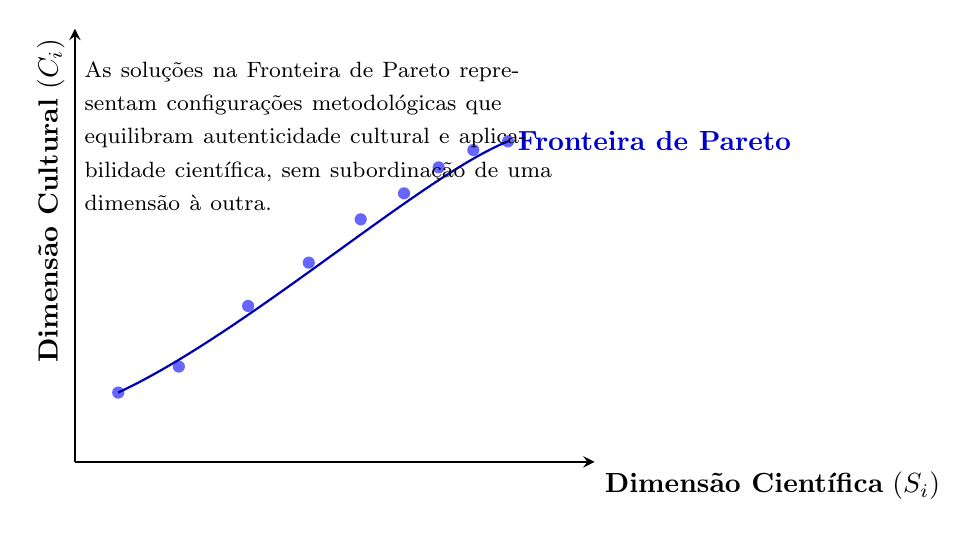
\begin{tikzpicture}[scale=1.1,>=stealth]
    % Eixos
    \draw[->, thick] (0,0) -- (6,0) node[below right]{\textbf{Dimensão Científica} ($S_i$)};
    \draw[->, thick] (0,0) -- (0,5) node[above left, rotate=90]{\textbf{Dimensão Cultural} ($C_i$)};
    
    % Pontos e fronteira
    \foreach \x/\y in {0.5/0.8, 1.2/1.1, 2.0/1.8, 2.7/2.3, 3.3/2.8, 3.8/3.1, 4.2/3.4, 4.6/3.6, 5.0/3.7} {
        \fill[blue!60] (\x,\y) circle (2pt);
    }
    \draw[thick, blue!70!black] (0.5,0.8) .. controls (2,1.5) and (4,3.3) .. (5,3.7);
    \node[blue!80!black, right] at (5,3.7) {\textbf{Fronteira de Pareto}};
    
    % Legenda
    \node[align=left, text width=6cm, below right, yshift=-0.3cm] at (0,5) {
        \footnotesize As soluções na Fronteira de Pareto representam configurações metodológicas que equilibram autenticidade cultural e aplicabilidade científica, sem subordinação de uma dimensão à outra.
    };
\end{tikzpicture}
\caption{Representação esquemática da Fronteira de Pareto cultural–científica obtida pelo algoritmo NSGA-II.}
\label{fig:pareto_nsga}
\end{figure}


\newpage